\section{Quantum error correction}
    Why do we use quantum error correction? Classical computers have some errors but quantum computers have much higher rates of errors (noise).
    \subsection{Classical error correction}
        One solution is \important{redundancy}: you encode n bits of information in m bits (m > n).
        \begin{remark}{Example}
            \begin{tcolorbox}[rouge]
                Let's suppose I want to send 1 bit over a noisy channel. 

                \textbf{Encoding:}
                \begin{align*} 
                    1 &\to 111 \\
                    0 &\to 000.
                \end{align*}
                Here $n =1$ and $m=3$.

                \textbf{Decoding:}
                
                Majority vote, $\bar{m}=abc \to $ output, whichevere bit is in the majority.
            \end{tcolorbox}
        \end{remark}
    \subsection{Model of quantum communication}
        \begin{center}
        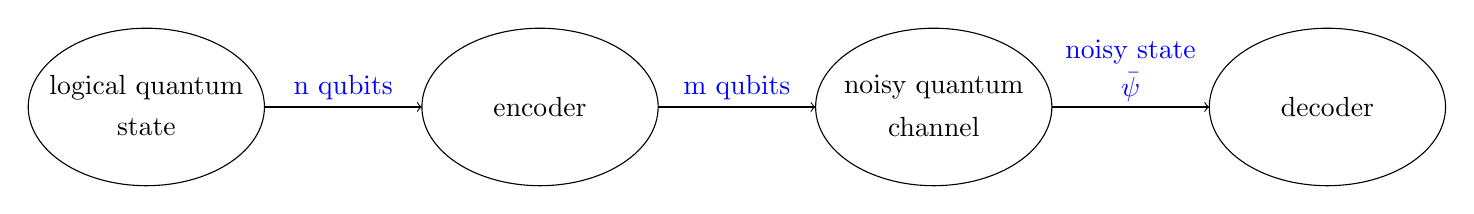
\begin{tikzpicture}
            \draw[thin] (-1,0) ellipse [x radius=1.5, y radius=1];
            \node at (-1, 0.25) {logical quantum};
            \node at (-1, -0.25) {state};
            \draw[thin] (4,0) ellipse [x radius=1.5, y radius=1];
            \node at (4, 0) {encoder};
            \draw[thin] (9,0) ellipse [x radius=1.5, y radius=1];
            \node at (9, 0.25) {noisy quantum};
            \node at (9, -0.25) {channel};
            \draw[thin] (14,0) ellipse [x radius=1.5, y radius=1];
            \node at (14, 0) {decoder};
            \draw[->, black] (0.5,0) -- (2.5,0);
            \node[blue] at (1.5, 0.25) {n qubits};
            \draw[->, black] (5.5,0) -- (7.5,0);
            \node[blue] at (6.5, 0.25) {m qubits};
            \draw[->, black] (10.5,0) -- (12.5,0);
            \node[blue] at (11.5, 0.7) {noisy state};
            \node[blue] at (11.5, 0.25) {$\ket{\bar{\psi}}$};
        \end{tikzpicture}
        \end{center}
    \subsection{Types of (single-qubit) quantum errors}
        \begin{itemize}[left=10pt, label=\textbullet]
            \item \textbf{X = bit flip error:} 
            \[X=\begin{pmatrix} 0 & 1 \\ 1 & 0 \end{pmatrix}, \mathspace \mathspace X\ket{0}=\ket{1}, \mathspace\mathspace X \ket{1}=\ket{0}, \mathspace\mathspace X\left(\alpha\ket{0}+\beta\ket{1}\right) = \alpha\ket{1}+\beta\ket{0}.\]
            
            \item \textbf{Z = phase flip error:}
                \[Z\ket{0}=\ket{0}, \mathspace\mathspace Z\ket{1}=-\ket{1}, \mathspace\mathspace Z\left(\alpha\ket{0}+\beta\ket{1}\right)=\alpha\ket{0}-\beta\ket{1}.\]
                \item \textbf{$R_{\theta}$ = Phase rotation:}
                    \[R_{\theta}=\begin{pmatrix} e^{-i\theta} & 0 \\ 0 & e^{i\theta} \end{pmatrix} .\]
        \end{itemize}
        \textbf{How quantum error correction differ form classical error correction:}
        \begin{itemize}[left=10pt, label=\textbullet]
            \item  The no-cloning theorem forbids copying information. 
            \item We can't look at quantum states and figure out which copy is wrong.
            \item There are infinately many types of quantum errors. For example 
                \[R_{\theta}, \mathspace\mathspace \theta \sim \left[0,2\pi\left[  \mathspace\mathspace \to \text{ continuous}\]
                    \item We have Y errors on top of X and Z errors. Recall: 
                    \[X =\begin{pmatrix} 0 & 1 \\ 1 & 0 \end{pmatrix}, \mathspace \mathspace Y = \begin{pmatrix} 0 & -i \\ i & 0 \end{pmatrix}, \mathspaces \mathspace Z = \begin{pmatrix} 1 & 0 \\ 0 & -1 \end{pmatrix} .\]
        \end{itemize}


    \subsection{Detection and correction of bitflip errors}
        \textbf{Encoding:} Quantum repetition code 
        \begin{align*} 
            \ket{0} \mathspace &\to \mathspace \ket{000}, \\
            \ket{1} \mathspace &\to \mathspace \ket{000}, \\
            \ket{\psi} = \alpha\ket{0}+\beta\ket{1} \mathspace &\to \mathspace \alpha\ket{000}+ \beta\ket{111}.
        \end{align*}
        \begin{center}\includegraphics[width=5cm]{images/2.png} \end{center}
        \textbf{Decoding:} The idea is to check parity of every neibhouring pair
        \begin{center}\includegraphics[width=9cm]{images/3.png} \end{center}

        We assume that there was at most one error.
        \begin{center}
            \begin{tabular}{c|c|c}
                \textbf{a}& {\textbf{b}} & which qubit had error\\  % ligne 1
                  \hline
                0 & 0 & none \\  
                    \hline
                0 & 1  & 3 \\
                    \hline
                1 & 0 & 1  \\
                      \hline
                1 & 1 & 2
            \end{tabular}
            \end{center}
        But at the end, this QECC is not satisfying, because
        \begin{itemize}[left=10pt, label=\textbullet]
            \item It only handles one error out of 3 possible error locations. 
            \item You use 3 qubits to protect one 1 qubit (inefficient). 
            \item It only works for one type of error (bitflip).
        \end{itemize}
        To counter the third point, we will see phaseflip code a 9-qubit Shor code.
    \subsection{Detection and correction of phaseflip errors}
        The key fact in phaseflip detection and correction error is that phaseflip is a bitflip in a different basis.

        We already seen the effect of Pauli's matrices X and Z on base $\{\ket{0}; \ket{1}\}$, now let's see the effect on Hadamard basis $\{\ket{+}; \ket{-}\}$:
        \begin{itemize}[left=10pt, label=\textbullet]
            \item $X\ket{+} = X\left(\frac{\ket{0}+\ket{1}}{\sqrt{2}}\right)=\frac{\ket{1}+\ket{0}}{\sqrt{2}}=\ket{+}$, 
            \item $X\ket{-} = X\left(\frac{\ket{0}-\ket{1}}{\sqrt{2}}\right)=\frac{\ket{1}-\ket{0}}{\sqrt{2}}=-\ket{-}$, 
            \item $Z\ket{+} = Z\left(\frac{\ket{0}+\ket{1}}{\sqrt{2}}\right)=\frac{\ket{0}-\ket{1}}{\sqrt{2}}=\ket{-}$, 
            \item $Z\ket{-} = Z\left(\frac{\ket{0}-\ket{1}}{\sqrt{2}}\right)=\frac{\ket{0}+\ket{1}}{\sqrt{2}}=\ket{+}$, 
        \end{itemize}
        Phaseflip error is a bitflip error in Hadamard basis!
        \begin{tcolorbox}[vert]
            Let H be the change matrice between $\ket{0}\slash \ket{1}$ basis and $\ket{+} \slash \ket{-}$ basis, then 
            \begin{itemize}[left=10pt, label=\textbullet]
                \item $H\ket{0}=\ket{+}$, 
                \item $H\ket{1}=\ket{-}$, 
                \item $H\ket{+}=\ket{0}$, 
                \item $H\ket{-}=\ket{1}$,
                \item $HXH = Z$, 
                \item $HZH = X$.
            \end{itemize}
        \end{tcolorbox}
        \begin{center}
        \includegraphics[width=10cm]{images/4.png}
        \end{center}
        $\text{E}_{\text{phase}} =$ phase where phaseflip error occurs.   
        
       \noindent \textbf{Explanation:} The idea here is to apply bitflip encoding circuit, then change in Hadamard basis before the error phase, change in normal basis and apply bitflip decoding circuit.

       But what if we have both bitflip and phaseflip errors at the same time?
    \subsection{9-qubit Shor code}
        9-qubit Shor code is just a code concatenation: 

        \textbf{Phaseflip encoding:} 
        \begin{align*} 
            \ket{0} &\to \ket{+++}, \\
            \ket{1} &\to \ket{---}.\\
        \end{align*}

        \textbf{Bitflip encoding:} 
        \begin{align*} 
            \ket{0} &\to\ket{000}, \\
            \ket{1} &\to \ket{111}.
        \end{align*}

        \textbf{Shor encoding:}
        \begin{align*} 
            \ket{0} \to \ket{000} \to \ket{+++} &\to \frac{1}{\sqrt{8}}\left(\ket{000}+\ket{111}\right)^{\otimes 3}, \\
            \underbrace{\ket{1} \to \ket{111} \to \ket{---}}_{\text{Phaseflip encoding}} &\to \underbrace{\frac{1}{\sqrt{8}}\left(\ket{000}-\ket{111}\right)^{\otimes 3}}_{\text{Bitflip encoding}}.
        \end{align*}
        \begin{center}
        \includegraphics[width=12cm]{images/5.png}
        \end{center}
        
        \begin{remark}{Apparté}
            Something important in QECC, is that quantum errors can be discretized, it means that: \important{correcting X,Y,Z} errors suffices to correct all quantum errors (though there are infinitely many).
            
            \vspace{1em}
            \textbf{Proof by example of Shor code:}

            Suppose we had $R_{\theta \text{ error}} = \cos \theta - i\sin \theta Z$, then errored encoded state: $\ket{\widetilde{\psi}}=R_{\theta}\ket{\widetilde{\psi}}=\cos \theta \ket{\bar{\psi}}-i\sin \theta Z \ket{\bar{\psi}}$.

            After applying the Shor code detection circuit: 
            \[\cos \theta \ket{\bar{\psi}}\ket{I}_{\text{SYN}}-i\sin \theta Z \ket{ \bar{\psi}}\ket{Z}_{\text{SYN}} \to \text{meas. syndrome register} \begin{functionbypart}{\to}
                \ket{\bar{\psi}}\ket{I}_{\text{SYN}} \text{ if }= \cos^2  \\
                Z\ket{\bar{\psi}}\ket{Z}_{\text{SYN}} \text{ if }= \sin^2
            \end{functionbypart}
            \]
            Note: now the syndrome register is entangled with the system registers.
        \end{remark}
        \textbf{Decoder:}

        Let 
        \begin{align*} 
            \ket{0} &\to \ket{+++} \to \left(\frac{\ket{000}+\ket{111}}{\sqrt{2}}^{\otimes3}\right)=\ket{\bar{0}}, \\
            \ket{1} &\to \ket{---} \to \left(\frac{\ket{000}-\ket{111}}{\sqrt{2}}^{\otimes3}\right)=\ket{\bar{1}}.
        \end{align*}
        \begin{enumerate}[left=10pt]
            \item Suppose that only one bitlflip happened, then the bitlfip decoder will decode as usual. 
            \item Suppose that only one phaseflip happened, then errored state is 
            \[\frac{1}{\sqrt{8}}\left(\ket{000}+\ket{111}\right)\left(\ket{000}-\ket{111}\right)\left(\ket{000}-\ket{111}\right),\]
            and the U decoder will decode with ``parity comparison for signs'' between the blocks. It will result as 
            \[\ket{+}\ket{0}\ket{0} \text{ for the first block, }\ket{-}\ket{0}\ket{0} \text{ for the second and } \ket{-}\ket{0}\ket{0} \text{ for the third.}\] 
            \item Suppose that both $X_1$ and $Z_1$ happened, the errored state is 
            \[\left(\ket{100}+\ket{011}\right)\left(\ket{000}-\ket{111}\right)\left(\ket{000}-\ket{111}\right),\]
            \begin{itemize}[left=10pt, label=\textbullet]
                \item Check for bitflip error \textrightarrow correct the bitflip error: $\left(\ket{000}+\ket{111}\right)\left(\ket{000}-\ket{111}\right)\left(\ket{000}-\ket{111}\right)$. 
                \item Check for phaseflip error \textrightarrow correct the phaseflip error.
            \end{itemize}
        \end{enumerate}
        The Shor code can also decode \important{some} 2-qubit errors, consider now this 2 qubits errors $X_1, X_2$. I claim there is no way to correct this error, why? 
        \begin{align*} 
            \text{It works with } \ket{\bar{0}} \text{ because:} \underbrace{\left(\ket{110}+\ket{001}\right)}_{\text{it will think error is on }X_3} &\xrightarrow{\text{after correction}} \left(\ket{111}+\ket{000}\right)=\left(\ket{000}+\ket{111}\right), \\
            \text{but not on } \ket{\bar{1}} \text{ because:} \underbrace{\left(\ket{110}-\ket{001}\right)}_{\text{it will think error is on }X_3} &\xrightarrow{\text{after correction}}\left(\ket{111}-\ket{000}\right) = -\ket{\bar{1}} = e^{i \phi} \text{ if } \phi = \pi, \ket{\bar{1}} \equiv \ket{\bar{1}}, \\
            \text{ BUT } &\alpha\ket{\bar{0}} + \beta\ket{\bar{1}} \neq \alpha\ket{\bar{0}} - \beta\ket{\bar{1}}.
        \end{align*}
    \subsection{Quantum code distance}
        \textbf{Recall:}

        The classical code distance is the minimum number of bits you need to flip to get from any codeword to any other codeword. Code distance relates to how many bitflip errors a classical code can correct $ \implies \lfloor\frac{\text{disance }-1}{2}\rfloor$.
        \begin{remark}{Example}
            \begin{tcolorbox}[rouge]
                $\{000, 111\} \implies $ number of correctable errors $ =1$, 
                \[000 \xrightarrow{\text{2 errors}} 011 \text{ will be closer to }111.\]
            \end{tcolorbox}
        \end{remark}
        \begin{tcolorbox}[vert]
             The Pauli weight is the number of positions where the is a non-I Pauli matrice $\sim$ quantum analog of the number of bitlfips.

            \noindent e.g. $XIX \to \text{ weight } = 2$.
        \end{tcolorbox}
        If $\ket{\bar{\psi_1}}, \mathspace \ket{\bar{\psi_2}}$ are two encoded statesw in the same code and $\exists \text{ Pauli }P \text{ s.t. } \ket{\bar{\psi_1}}=P\ket{\bar{\psi_2}}$, then Pauli P is \important{uncorrectable} because it looks just like ``no error on $\ket{\bar{\psi_1}}$''. 
        \begin{align*} 
         \text{Quantum code distance }:= \text{ min weight}\left(P\right) \text{ s.t. } P\ket{\bar{\psi_1}}=\ket{\bar{\psi_2}}, \\    
            \mathspace P = \text{ some Pauli string}, \mathspace \ket{\bar{\psi_1}}, \ket{\bar{\psi_2}} \text{ any two orthogonal code}.
        \end{align*}
        Analogous to classical code distance, quantum code with distance d can correct Pauli errors of weights at most $\left\lfloor \frac{d-1}{2} \right\rfloor $.
        \begin{remark}{Example}
            \begin{tcolorbox}[rouge]
                \begin{itemize}[left=10pt, label=\textbullet]
                    \item $n = \#$ of physical qubits (n-qubit codeword), 
                    \item $k = \#$ of logical qubits (to encode a k-qubit quantum state), 
                    \item $d:$ code distance.
                \end{itemize}
                \[\mathcal{H}_k \to \text{ ENC } \to \mathcal{H}_n,\]
                Shor's 9-qubit encode a single qubit into 9 qubit so it's a $\underbrace{\left[\left[n,k,d\right]\right]}_{9,1,3}$, that's why it can correct \important{all} errors of Pauli weight $\left\lfloor \frac{3-1}{2} \right\rfloor $.
            \end{tcolorbox}
        \end{remark}
        \textbf{What properties we want of a good QECC:}
        \begin{itemize}[left=10pt, label=\textbullet]
            \item make d as large as possible,
            \item $\frac{k}{n}$ as large as possible, 
            \item fast encoding (decoding).
        \end{itemize}
        \newpage
        Let $\left(U, \Sigma\right)$ be a QECC where $U: \mathcal{H}_K \to \mathcal{H}_N$ a map and $\Sigma$ is a set of correctable errors s.t. $\forall E \in \Sigma, \forall \ket{ \psi} \in \mathcal{H}_K$, there is a decoding map that restores the errored state: $D\left(EU\ket{\psi}\bra{\psi}U^{\dagger}E^{\dagger}\right) \propto \ket{\psi}\bra{\psi}$. 
        \begin{theoreme}
            If $\left(U, \Sigma\right)$ is a QECC then $\left(U, span\left(\Sigma\right)\right)$ is also a QECC. Then, to correct arbitrary errors like $\alpha E+ \beta F$, it suffices to correct $E,F \implies$ \important{quantum errors can be discretized!}
        \end{theoreme}
    \subsection{Fault tolerance and error propagation}
        We've seen ways to encode quantum states such that any error can be detected and corrected. But how do we act with gates in a way that doesn't propagate errors? \textrightarrow $\mathspace$\important{fault tolerance}.

    \noindent Moreover, we've assumed that encoding/decoding are noiseless, but they also suffer from noise. The main idea will be: we only decode information when absolutely necesseray.
    \begin{remark}{Example}
        \begin{tcolorbox}[rouge]
            Suppose I want to carry out $\ket{0}\xrightarrow{H}\ket{+}$.

            \textbf{Silly way:} 
            \[\ket{0}\to \text{Enc} \to \ket{\bar{0}} \to \text{Noise} \to \text{Dec} \to H \to \text{Enc} \to \text{Noise} \to \text{Dec} \to \ket{+}.\]
            \noindent \textbf{Instead:} 
            \[\ket{0}\to\text{Enc}\to\ket{\bar{0}}\to \bar{H}\to\ket{\bar{+}} \to \text{Dec}\to \ket{+}.\]
            This saves one cycle of decoding and encoding.
        \end{tcolorbox}
    \end{remark}
    Recall that encoding means going to a larger Hilbert space. So encoded operations also have to act on a larger Hilbert space.

    \noindent Key idea: we encode gates in a way that doesn't spread errors.

    Let 
    \begin{center}
    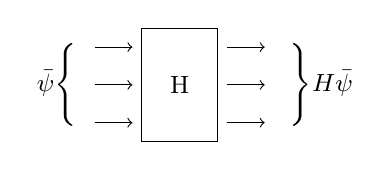
\begin{tikzpicture}[scale=1.2, every node/.style={font=\small}]
        \draw [draw=black] (1.1,1.5) rectangle (0.3,0.3);
        \node at (0.7, 0.9) {H};
        \draw[->, black]
            (-0.2,1.3) -- (0.2,1.3);
        \draw[->, black]
            (-0.2,0.5) -- (0.2,0.5);
        \draw[->, black]
            (-0.2,0.9) -- (0.2,0.9);
        \node at (-0.6, 0.9) {$\ket{\bar{\psi}}\Biggl\{$ };
        \draw[->, black]
            (1.2,0.9) -- (1.6,0.9);
        \draw[->, black]
            (1.2,1.3) -- (1.6,1.3);
        \draw[->, black]
            (1.2,0.5) -- (1.6,0.5);
        \node at (2.2, 0.9) {$\Biggr\}\ket{H\ket{\bar{\psi}}}$};
    \end{tikzpicture}
    \end{center}
    What operations should go insinde the box?

    Option 1: 
    \begin{center}
    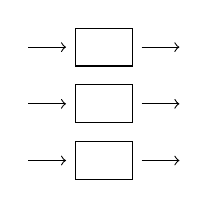
\begin{tikzpicture}[scale=1.2, every node/.style={font=\small}]
         \draw[->, black]
            (-0.8,-0.1) -- (-0.4,-0.1);
        \draw [draw=black] (0.3,0.1) rectangle (-0.3,-0.3);
        \draw[->, black]
            (0.4,-0.1) -- (0.8,-0.1);

        \draw[->, black]
            (-0.8,-0.7) -- (-0.4,-0.7);
        \draw [draw=black] (0.3,-0.5) rectangle (-0.3,-0.9);
        \draw[->, black]
            (0.4,-0.7) -- (0.8,-0.7);


        \draw[->, black]
            (-0.8,-1.3) -- (-0.4,-1.3);
        \draw [draw=black] (0.3,-1.1) rectangle (-0.3,-1.5);
        \draw[->, black]
            (0.4,-1.3) -- (0.8,-1.3);
    \end{tikzpicture}
    \end{center}
    Option 2:
    \begin{center}
    \begin{tikzpicture}[scale=1.2, every node/.style={font=\small}]
         \draw[->, black]
            (-0.8,-0.1) -- (-0.4,-0.1);
        \draw [draw=black] (0.3,0.1) rectangle (-0.3,-0.9);
        \draw[->, black]
            (0.4,-0.1) -- (1.8,-0.1);
        \draw[->, black]
            (-0.8,-0.7) -- (-0.4,-0.7);
        \draw[->, black]
            (0.4,-0.7) -- (0.8,-0.7);

        \draw[->, black]
            (-0.8,-1.3) -- (0.8,-1.3);
        \draw [draw=black] (0.9,-0.5) rectangle (1.5,-1.5);
        
        \draw[->, black]
            (1.6,-0.7) -- (1.8,-0.7);
        \draw[->, black]
            (1.6,-1.3) -- (1.8,-1.3);
    \end{tikzpicture}
    \end{center}
    \textbf{Reasons to prefer option 1:}
    \begin{itemize}[left=10pt, label=\textbullet]
        \item Most hardware platforms ahve much higher fidelity for single qubit gates than for multiple qubit gates. 
        \item Transversal gates are ``better'' for preventing propagation.
    \end{itemize}
    \textbf{Transversal gates:}

    Defining a code block $\left[\left[n,k,d\right]\right]$,
    \begin{tcolorbox}[vert]
        Transversality means that each encoded gate touches 1 qubit from each code block.
    \end{tcolorbox}
    Transversality ensures that if any error occurs, the gate can propagate it to at most one error per block.


